%% ============================================================================
%% DRAFT assembled from verified materials (research-brief, experiment-plan,
%% results/, notes/sources.md, paper/related-work.md). The AUTHOR owns the
%% argument, the interpretation, and the final voice; this is a draft from
%% direction to be revised. Every citation is verified (see notes/sources.md).
%% All numbers are taken verbatim from results/tables/<dataset>/.
%% Target: arXiv preprint, ACM acmart numeric. Compile: pdflatex; bibtex; pdflatex x2.
%% ============================================================================
\documentclass[sigconf,nonacm]{acmart}
\settopmatter{printacmref=false}
\citestyle{acmnumeric}
\setcopyright{none}
\pagestyle{plain}
% Figures live in paper/figures/ (self-contained). Regenerate with experiment/make_figures.py.
% To submit: upload this paper/ folder (main.tex, references.bib, figures/) to arXiv/Overleaf.
\graphicspath{{figures/}}

\begin{document}

\title{Responsible AI Through Data Quality: Group-Correlated Missingness as an
Upstream, Pipeline-Placed Fairness Check}

\author{Bijaya Shrestha}
\affiliation{\institution{Independent Researcher}\country{}}
\email{shrestha.bj2056@gmail.com}

\renewcommand{\shortauthors}{Shrestha}

\begin{abstract}
Most machine-learning fairness work intervenes at the \emph{model}. We argue that an
important class of fairness harm can be detected \emph{upstream}, in the data pipeline,
before a model is trained. We study \emph{group-correlated missingness}---missing data whose
rate differs across a protected attribute---as a cheap, model-free signal, and make the
contribution operational along three legs: (1)~a concrete \emph{missingness-disparity
statistic} ($D_{\max}$, the maximum across features of the between-group missingness-rate
gap); (2)~a controlled benchmark that tests whether $D_{\max}$, measured before training,
\emph{predicts} the post-training equalized-odds gap; and (3)~a \emph{validation-stage gate}
that implements the check inside an existing data-quality framework. Across three public
datasets the signal is \emph{demonstrated but bounded}, and mapping that boundary is a central
result. On Adult the pre-training statistic predicts the baseline-corrected equalized-odds gap
(Pearson $r\approx0.40$, rising to $0.52$ under MNAR; early-warning AUROC up to $0.78$), more
cleanly than demographic parity. On COMPAS the relationship \emph{reverses}; a controlled
encoding-flip experiment shows this is not noise or an artifact but a \emph{boundary condition}
---the sign is governed by which group carries the excess missingness (positive when it falls on
the smaller / lower-base-rate group), flipping in both datasets when the encoding is flipped. On
German Credit the correlation is \emph{null}, exposing a second, orthogonal axis: at $n{=}1000$
the effect is swamped by equalized-odds estimation noise, so detectability requires sufficient
data. We also derive the gate's decision threshold from the benchmark (F1-optimal $D_{\max}\approx
0.10$ on Adult) and characterize the gate as a high-recall screen. We release a reproducible
three-dataset benchmark and a runnable gate (with an executed Great Expectations integration;
Deequ/TFDV adapters are interface-compatible but not executed), positioning missingness-aware
fairness checking as a data-engineering problem whose reach we bound honestly.
\end{abstract}

\keywords{fairness, missing data, data quality, data validation, machine-learning pipelines,
equalized odds}

\maketitle

\section{Introduction}
Fairness interventions in machine learning predominantly target the model: reweighing,
constrained training, post-processing of scores. Yet many fairness harms originate in the
data, and a recurring observation is that \emph{missing data} in particular has been
neglected as a fairness concern~\cite{martinezplumed2021}. This paper takes a
data-engineering stance: rather than measuring unfairness after a model exists, we ask what
can be measured at ingestion or transformation time, and where such a check belongs in the
pipeline.

Our object of study is \emph{group-correlated missingness}: missingness whose rate is
correlated with a protected attribute. The premise that such missingness can harm downstream
fairness is established~\cite{goel2021,wangsingh2021,min2025}. Our contribution is not that
premise but its \emph{operationalization}, along three legs that must all hold or the work
reduces to something already done:
\begin{enumerate}
\item \textbf{A validated statistic.} $D_{\max}$, a concrete group-wise
missingness-disparity statistic, computed pre-training and model-free
(Section~\ref{sec:stat}).
\item \textbf{Predictive validity.} Empirical evidence, on controlled benchmarks, that
$D_{\max}$ forecasts equalized-odds degradation \emph{before} training---together with an
honest characterization of where it fails (Sections~\ref{sec:method}--\ref{sec:results}).
\item \textbf{Pipeline placement.} The check implemented as a pre-training validation gate
inside an existing data-quality framework, the leg that makes it a data-engineering artifact
(Section~\ref{sec:gate}).
\end{enumerate}
We frame the work as the pipeline operationalization that recent audit-oriented
work~\cite{mdla2026} calls for but does not build. Equally central is where the signal
\emph{fails}: across three datasets we find it holds on Adult, reverses on COMPAS, and vanishes
on German Credit, and we identify the two properties---group structure and sample size---that
govern which regime obtains. The honesty of that boundary is a contribution, not a caveat.

\section{Related Work}\label{sec:related}
\textbf{Data quality as a fairness concern.}
A recurring theme is that fairness harms originate in data. Mart\'inez-Plumed et
al.~\cite{martinezplumed2021} argue missing values are a neglected dimension of fairness;
surveys catalogue the standard group-fairness metrics and the impossibility results among
them~\cite{caton2024}, context for our deliberate commitment to equalized odds.

\textbf{Missingness and fairness.}
The link is established. Goel et al.~\cite{goel2021} show via causal graphs that ignoring
missingness can nullify fairness guarantees; Wang and Singh~\cite{wangsingh2021} show missing
values and selection bias shift fairness even when accuracy is stable; Min et
al.~\cite{min2025} provide peer-reviewed evidence that disparities worsen ``even for little
missingness.'' Responses are predominantly model-level or post-hoc: Jeong et
al.~\cite{jeong2022} propose an in-processing fair decision tree (Fair MIP Forest) that
incorporates missingness as an attribute and optimizes equalized odds without imputation;
Feng et al.~\cite{feng2023} adapt fairness interventions to missing patterns and show that
naive impute-then-classify can \emph{worsen} group fairness---a result we rely on to justify
holding imputation fixed rather than treating it as the remedy. A genuine tension exists:
Bhatti et al.~\cite{bhatti2025} (preprint) report that the missingness \emph{mechanism} does
not significantly move fairness at high missingness, whereas the works above find clear
effects. We read these as compatible---mechanism \emph{type} versus presence and
group-correlation of missingness---and design our benchmark to characterize the regime in
which the signal holds.

\textbf{Data-validation tooling.}
Mature frameworks guard production pipelines but carry no group-wise notion: Deequ provides
declarative completeness and null-rate constraints~\cite{schelter2018deequ}; TensorFlow Data
Validation~\cite{caveness2020} and Great Expectations~\cite{greatexpectations} provide schema-
and expectation-based gates. Pipeline-aware fairness tooling is diagnostic rather than
predictive: mlinspect inspects operators post hoc for distribution and technical-bias
issues~\cite{grafberger2022}; FairPrep promotes data to first-class in fairness-intervention
studies~\cite{schelter2020fairprep}; Biswas and Rajan analyze how preprocessing-stage fairness
composes~\cite{biswasrajan2021}. We add a single fairness-relevant, \emph{predictive} check to
this class of gate.

\textbf{Closest competitors.}
The Missingness Demographic Leakage Audit~\cite{mdla2026} (preprint) is a manual, four-step
retrospective \emph{audit} on ICU data testing whether missingness indicators leak demographics;
its findings are associative, and its response is post-hoc recalibration. It shares our
pre-deployment stance, so the distinction is not timing but \emph{operationalization}: MDLA does
not automate the check into a pipeline validation gate, nor calibrate a threshold that
\emph{forecasts} downstream fairness degradation---the prospective evaluation it lists as future
work, and what we build.
Su\'arez Ferreira et al.~\cite{suarezferreira2025} (preprint) propose a data-centric early
indicator of fairness, but the signal is classification \emph{complexity}, not missingness,
and they address neither pipeline placement nor automation.

\section{The Missingness-Disparity Statistic}\label{sec:stat}
Let $g\in\{0,1\}$ denote a binary protected attribute and let $m_f(g)$ be the missingness
rate of feature $f$ within group $g$. The per-feature disparity is
$\delta_f = |m_f(1)-m_f(0)|$. Our primary statistic aggregates by the maximum:
\[
D_{\max} = \max_f\,\big|\,m_f(1)-m_f(0)\,\big|.
\]
$D_{\max}$ is cheap, interpretable (it flags the single worst feature), and---crucially---
needs neither the target nor a fitted model, so it can run at a true pre-label ingestion gate.
We also consider a \texttt{mean} aggregation, a \texttt{weighted} aggregation (by per-feature
missingness prevalence), and an importance-aware \texttt{mi\_weighted} aggregation that weights
each $\delta_f$ by the feature's mutual information with the target; the latter is still
model-free (no model is fit), preserving the ingestion-time property.

\section{Predictive-Validity Benchmark}\label{sec:method}
\textbf{Design.} Starting from (near-)complete public data, we \emph{inject} missingness so
that the mechanism and group-correlation are known---the control real data cannot give. We
vary three knobs: mechanism (MCAR / MAR / MNAR), between-group rate gap
$\{0,0.05,0.10,0.20,0.30\}$, and overall rate $\{0.05,0.15,0.30\}$, with ten seeds, for $450$
cells per dataset. Per cell we (1)~inject; (2)~compute $D_{\max}$ on the injected training data
(the upstream check); (3)~impute with a fixed strategy (median) held constant so imputation is
not a confound; (4)~train a fixed logistic-regression model; and (5)~measure the
equalized-odds gap (primary) and demographic-parity gap (secondary) on a held-out test set.

\textbf{Target.} Because a dataset's inherent unfairness dominates the absolute gap, our
primary target is the \emph{baseline-corrected} equalized-odds gap, $\Delta_{\mathrm{EO}}$:
the cell's gap minus that of its matching no-disparity cell (same mechanism, rate, seed, with
zero rate gap). This isolates the contribution of group-correlated missingness from both the
dataset's baseline unfairness and from missingness that is present but not group-correlated.
We report equalized odds as primary (the causal story---uneven corruption yields uneven error
rates---maps onto error-rate fairness) and name the fairness impossibility
results~\cite{caton2024} so the equalized-odds-specific framing is deliberate.

\textbf{Datasets.} Three public datasets of deliberately different size and domain: Adult
(Census Income; protected attribute sex; $45{,}222$ complete rows), COMPAS (two-year
recidivism; race, Caucasian vs.\ African-American; $5{,}278$ rows), and German Credit
(Statlog; age $>25$; $1{,}000$ rows). The benchmark is fully reproducible from one command with
fixed seeds.

\section{Results}\label{sec:results}

\begin{figure*}[t]\centering
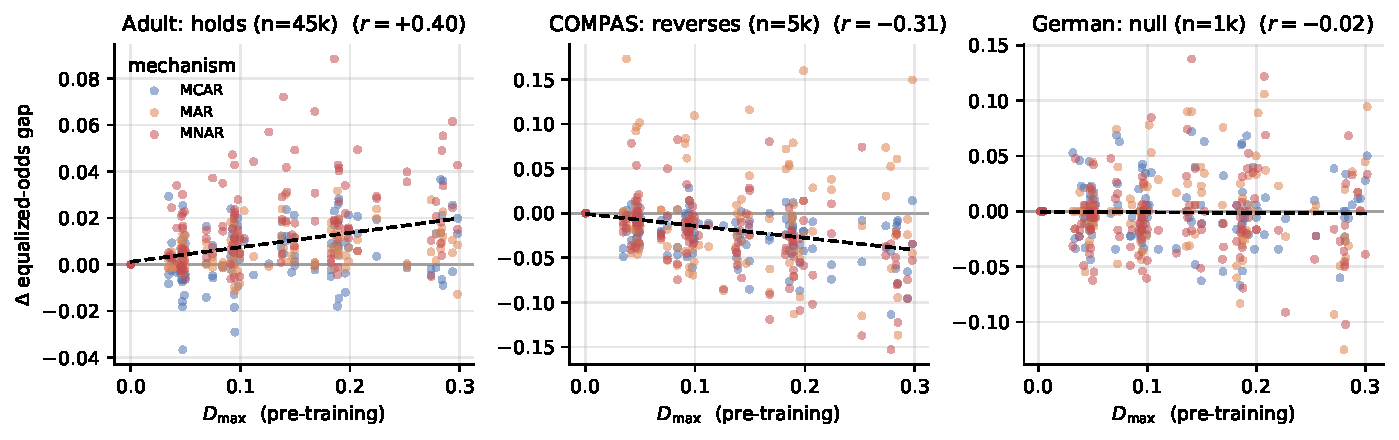
\includegraphics[width=0.92\textwidth]{fig1_scatter_contrast}
\caption{Pre-training $D_{\max}$ vs.\ the post-training baseline-corrected equalized-odds gap
across all 450 grid cells per dataset, coloured by mechanism. The relationship is positive on
Adult ($r=+0.40$), reverses on COMPAS ($r=-0.31$), and is null on German Credit ($r=-0.02$)---the
full generalization map. Sign and detectability are governed by group structure and sample size,
respectively (Sec.~\ref{sec:results}).}
\label{fig:contrast}
\end{figure*}

\textbf{Adult: the signal holds.} $D_{\max}$ predicts $\Delta_{\mathrm{EO}}$ with Pearson
$r=0.40$ pooled (Spearman $0.46$; Figure~\ref{fig:contrast}, left). The relationship is
strongest exactly where the thesis expects---under MNAR, which is also the most harmful
mechanism (Table~\ref{tab:regime}, Figure~\ref{fig:mech}). As an early-warning detector,
thresholding $D_{\max}$ to flag $\Delta_{\mathrm{EO}}$ exceedance gives AUROC $0.74$ (threshold
$0.02$) and $0.78$ (threshold $0.05$; Figure~\ref{fig:roc}). As expected, $D_{\max}$ predicts
the equalized-odds gap ($r=0.40$) more cleanly than demographic parity ($r=0.30$), and the
baseline correction is essential: against the \emph{absolute} equalized-odds gap the
correlation falls to $0.16$.

\begin{figure}[t]\centering
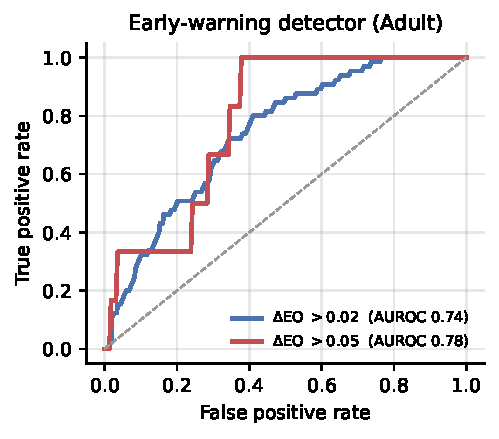
\includegraphics[width=0.84\columnwidth]{fig2_detector_roc}
\caption{Early-warning detector on Adult: ROC for flagging $\Delta_{\mathrm{EO}}$ exceedance by
thresholding the pre-training $D_{\max}$.}
\label{fig:roc}
\end{figure}

\begin{table}[t]\centering\small
\caption{Adult, by mechanism: $D_{\max}$ vs.\ $\Delta_{\mathrm{EO}}$ ($n=150$ each). MNAR is
the most harmful and the most predictable.}\label{tab:regime}
\begin{tabular}{lccc}
\toprule
mechanism & mean $\Delta_{\mathrm{EO}}$ & Pearson $r$ & Spearman \\
\midrule
MCAR & 0.004 & 0.34 & 0.29 \\
MAR  & 0.005 & 0.44 & 0.51 \\
MNAR & 0.015 & \textbf{0.52} & \textbf{0.61} \\
\bottomrule
\end{tabular}
\end{table}

\textbf{Aggregation.} The aggregation choice barely matters: $D_{\max}$ $r=0.398$, \texttt{mean}
$0.388$, \texttt{weighted} $0.401$, importance-aware \texttt{mi\_weighted} $0.418$. The
importance-aware variant is marginally best (Figure~\ref{fig:agg})---confirming that harm
depends on which features are disparate---but it requires the target at the gate, trading away
the no-labels property; we therefore keep $D_{\max}$ as the recommended default.

\begin{figure}[t]\centering
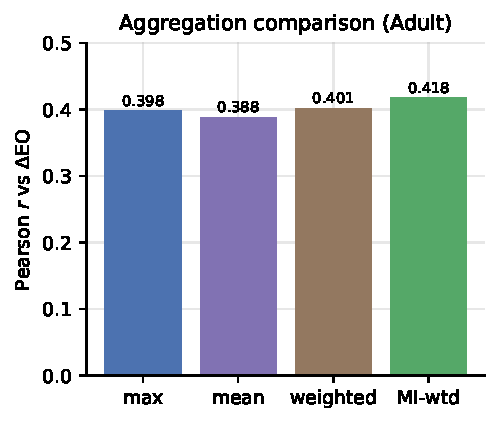
\includegraphics[width=0.84\columnwidth]{fig4_aggregation}
\caption{Aggregation comparison on Adult. All four aggregations of the disparity statistic
predict $\Delta_{\mathrm{EO}}$ comparably; the importance-aware MI-weighted variant is marginally
best. $D_{\max}$ is the labels-free default.}
\label{fig:agg}
\end{figure}

\textbf{COMPAS: the sign reverses---a boundary condition.} On COMPAS the relationship
\emph{reverses} (pooled $r=-0.31$). This is neither noise nor an artifact: the sign is robust to
injecting only the non-zero-inflated \texttt{age} feature ($-0.42$) and to mean imputation
($-0.22$). A controlled \emph{encoding-flip} experiment identifies the cause: flipping the
protected-group encoding---so the excess missingness falls on the other group---flips the sign of
$r$ in \emph{both} datasets (Adult $+0.40\!\rightarrow\!-0.36$; COMPAS $-0.31\!\rightarrow\!+0.42$),
with magnitude preserved (Figure~\ref{fig:flip}). The sign is therefore governed by \emph{which
group carries the excess missingness}: positive when it falls on the smaller / lower-base-rate
group, negative on the larger / higher-base-rate group. The statistic carries predictive signal in
every configuration ($|r|\approx0.4$); only the \emph{direction} of downstream harm depends on
group structure. Three structural properties (minority status, the sign of the base-rate
difference, and the sign of the protected--target correlation) co-vary across our two datasets, so
we cannot yet isolate which is causal.

\begin{figure}[t]\centering
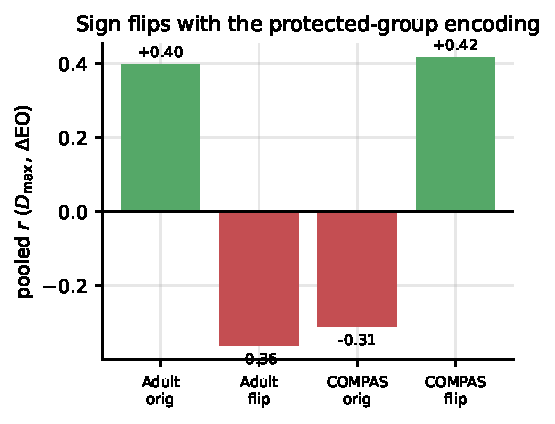
\includegraphics[width=0.80\columnwidth]{fig5_boundary_flip}
\caption{Encoding-flip test. Flipping which group carries the excess missingness flips the sign of
$r$ in both datasets, magnitude preserved---so the sign is a function of group structure, not
dataset identity.}
\label{fig:flip}
\end{figure}

\textbf{German Credit: null---a detectability limit.} On German Credit the correlation is null
($r=-0.02$), even though its structure predicts a positive sign by the rule above (the
unprivileged group is a minority with a lower base rate). The effect is not small---the mean
per-cell $|\Delta_{\mathrm{EO}}|$ ($0.020$) exceeds Adult's ($0.010$)---it is \emph{noise-dominated}:
at $n=1000$ (a $\sim$300-row test set) equalized-odds fluctuations swamp the injected disparity,
dissolving the linear signal. Detectability thus depends on sample size, a second axis orthogonal
to the sign. Together the three datasets map the boundary: the signal is present and
sign-predictable-by-structure when the sample is large enough (Adult, COMPAS) and undetectable when
it is not (German).

\begin{figure}[t]\centering
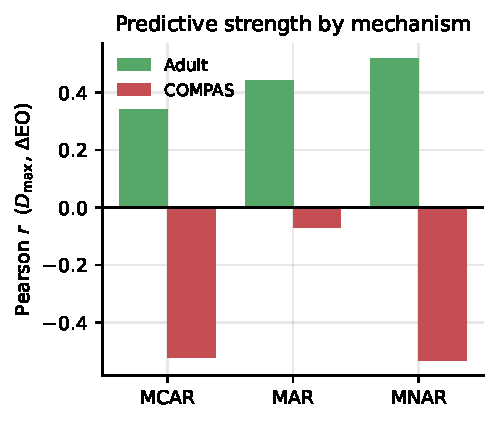
\includegraphics[width=0.84\columnwidth]{fig3_mechanism_r}
\caption{Predictive strength ($r$ between $D_{\max}$ and $\Delta_{\mathrm{EO}}$) by mechanism:
positive on Adult---strongest under MNAR---and negative across mechanisms on COMPAS.}
\label{fig:mech}
\end{figure}

\begin{figure*}[t]\centering
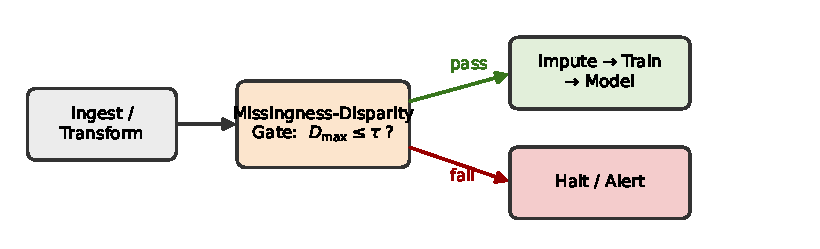
\includegraphics[width=0.86\textwidth]{fig0_gate_schematic}
\caption{The missingness-disparity gate at a pre-training validation stage. It computes
$D_{\max}$ on an incoming batch and halts (or alerts) when the value exceeds the policy threshold
$\tau$; otherwise the batch proceeds to imputation and training. The check needs only the
features and the protected-attribute label---no target and no model.}
\label{fig:gate}
\end{figure*}

\section{The Validation Gate}\label{sec:gate}
The statistic becomes a data-engineering artifact when placed at a pre-training validation
stage (Figure~\ref{fig:gate}). Our gate computes $D_{\max}$ on an incoming batch and fails the
pipeline when it exceeds
a policy threshold $\tau$; it requires only the features and the protected-attribute label---no
target, no model. We \emph{derive} $\tau$ from the benchmark rather than assert it: on Adult, the
F1-optimal cutoff for flagging a meaningful equalized-odds increase is $D_{\max}\approx0.10$
(recall $0.72$, precision $0.26$; a precision-$0.8$ operating point is unreachable). The gate is
thus best read as a \emph{high-recall screen}---a sensitive early warning that flags data for
review, not a precise oracle---which is the appropriate role for a validation gate and consistent
with a moderate predictor. The threshold is Adult-calibrated and, by the boundary condition above,
regime-dependent. On a batch with strong group-correlated missingness the gate fails
($D_{\max}=0.30 > \tau=0.10$, worst feature \texttt{age}); on a batch with the same overall
missingness but \emph{no} group correlation it passes ($D_{\max}=0.00$), on both Adult and COMPAS.

Data-validation frameworks such as Deequ~\cite{schelter2018deequ},
TFDV~\cite{caveness2020}, and Great Expectations~\cite{greatexpectations} natively measure
per-column completeness but carry no group-wise or fairness-linked notion. The integration
pattern is the same for each: let the framework measure the per-group, per-column null rate
(its native strength), compose those into $D_{\max}$, and enforce $\tau$ (the fairness leg they
lack). We implement and \emph{execute} the Great Expectations integration end to end---it routes
the per-group null measurement through the framework's own validation engine and reproduces the
gate decision. The Deequ and TFDV adapters are \emph{interface-compatible but not executed} here
(they require a Spark/JVM and a TensorFlow runtime, respectively); we provide them as reference
integrations against the documented APIs. This is what answers the ``just Deequ with a fairness
label'' critique: the gate is a \emph{demographic} disparity check with empirically
characterized predictive validity, not a bare null-rate constraint.

\section{Discussion and Limitations}\label{sec:discussion}
The claim is deliberately bounded, and mapping the boundary is part of the contribution. Across
three datasets the signal holds (Adult), reverses (COMPAS), and vanishes (German), and two axes
explain which regime obtains: its \emph{sign} is governed by group structure (the encoding-flip
result) and its \emph{detectability} by sample size (the German null). This is itself the
adjudication of the conflicting prior results~\cite{bhatti2025,min2025}. The main open question is
which of the three co-varying structural properties drives the sign; our two large-enough datasets
confound them, and a dataset in which they diverge would isolate the cause. We deliberately hold
imputation fixed---imputation choice is a known, separate fairness lever~\cite{feng2023}---and we
leave mitigation to future work: the gate \emph{detects}, it does not repair. Finally, our
protected attributes are binary; extending $D_{\max}$ to multi-group settings is straightforward in
principle but untested here.

\section{Conclusion}
Fairness harm from group-correlated missingness can be checked \emph{before} training with a
cheap, model-free statistic placed at a data-validation gate. On Adult the check predicts
equalized-odds degradation with useful early-warning performance, strongest under MNAR; on COMPAS
its sign reverses and on German it vanishes---and we show these are not failures of the method but
a boundary set by group structure and sample size. Treating fairness as an upstream data-quality
assurance problem---and building the check into the pipeline tooling engineers already run, with an
honest account of where it works---is the data-engineering contribution this paper makes concrete.

\section*{Reproducibility}
All benchmark data are public. One command (\texttt{python experiment/run\_all.py --dataset
all}) regenerates every figure and table from fixed seeds; the gate demonstration is
\texttt{python experiment/demo\_gate.py}. Code and verified references are released with the
paper.

\section*{Use of AI Tools}
During the preparation of this work the author used AI-assisted tools for literature search and
source triage, citation formatting, code scaffolding and debugging, and drafting from
author-provided direction. The author reviewed and edited all such output, independently
verified every cited source against its primary record, and takes full responsibility for the
argument, the interpretation, and the conclusions.

\bibliographystyle{ACM-Reference-Format}
\bibliography{references}

\end{document}
